%!TeX TXS-program:bibliography = txs:///biber
\documentclass{article}

% other stuff
\usepackage[dvipsnames]{xcolor}
\usepackage{fullpage}
\usepackage{graphicx}
\usepackage{authblk}
\usepackage{booktabs}
\usepackage[%
plainpages=false,%
colorlinks,% removes the boxes around links
urlcolor=black,%
filecolor=black,%
citecolor=Blue,%   requires xcolor with option dvipsnames
linkcolor=black,%
pdfpagemode=UseOutlines,%
pdfauthor={Lars Vilhuber},%
pdfsubject={Economics, Reproducibility, Open Science},%
]{hyperref}

\usepackage[
backend=biber,
authordate,
  noibid,
  natbib,
  sorting=nyt,
  sortcites=true
  abbreviate=false,
  citetracker=false,
  isbn=false,ibidtracker=false]{biblatex-chicago}

\defbibfilter{papers}{
     type=article or
     type=inproceedings or
     type=conference or
     type=proceedings or
     type=incollection or
     type=inbook
}
% Clear some stuff from the bibliography
\AtEveryBibitem{%
        \clearfield{day}%
        \clearfield{month}%
        \clearfield{endday}%
        \clearfield{endmonth}%
    \clearlist{language}%
    \clearfield{issn}%
    \clearfield{eprint}% - adjust if necessary
    \iffieldundef{doi}{}{\clearfield{url}}% remove URL field if DOI present    
}

% acronyms
\usepackage{acronym}

\acrodef{AEA}{American Economic Association}
\acrodef{AI}{artificial intelligence}
\acrodef{AJPS}{American Journal of Political Science}
\acrodef{BPLIM}{Banco de Portugal Microdata Research Laboratory}
\acrodef{BLS}{Bureau of Labor Statistics}
\acrodef{CASD}{Centre d'accès sécurisé aux données}
\acrodef{CC-BY}{Creative Commons Attribution}
\acrodef{CIQSS}{Centre interuniversitaire québécois de statistiques sociales}
\acrodef{CEA}{Canadian Economics Association}
\acrodef{CJE}{Canadian Journal of Economics}
\acrodef{CSWEP}{AEA Committee on the Status of Women in the Economics Profession}
\acrodef{DCAP}{data and code availability policy}
\acrodef{DCAS}{Data and Code Availability Standard}
\acrodef{DHS}{Demographic and Health Surveys}
\acrodef{DOI}{Digital Object Identifier}
\acrodef{EEA}{European Economics Association}
\acrodef{EJ}{Economic Journal}
\acrodef{EI}{Economic Inquiry}
\acrodef{ERS}{Economic Research Service}
\acrodef{FAIR}{Findable, Accessible, Interoperable, Re-usable}
\acrodef{FAQ}{frequently asked questions}
\acrodef{FSRDC}{Federal Statistical Research Data Centers}
\acrodef{GDPR}{General Data Protection Regulation}
\acrodef{GIS}{geographical information system}
\acrodef{GPU}{graphical processing unit}
\acrodef{HRS}{Health and Retirement Study}
\acrodef{IAB}{Research Data Center (FDZ) at the Institute for Employment Research}
\acrodef{IRS}{Internal Revenue Service}
\acrodef{IRB}{institutional review board}
\acrodef{ICPSR}{Inter-university Consortium for Political and Social Research}
\acrodef{JASA}{Journal of the American Statistical Association}
\acrodef{JEEA}{Journal of the European Economic Association}
\acrodef{JFE}{Journal of Financial Economics}
\acrodef{JPC}{Journal of Privacy and Confidentiality}
\acrodef{HDSR}{Harvard Data Science Review}
\acrodef{SPCR}{Society for Confidentiality and Privacy Research}
\acrodef{LLM}{large language models}
\acrodef{LMIC}{low- and middle-income countries}
\acrodef{NACJD}{National Archive of Criminal Justice Data}
\acrodef{NBER}{National Bureau of Economic Research}
\acrodef{NLSY}{National Longitudinal Survey of Youth}
\acrodef{OLDA}{Ohio Longitudinal Data Archive}
\acrodef{PAP}{pre-analysis plans}
\acrodef{PII}{personally identifiable information}
\acrodef{PSID}{Panel Study of Income Dynamics}
\acrodef{RAM}{random access memory}
\acrodef{RCT}{randomized control trial}
\acrodef{RePEc}{Research Papers in Economics}
\acrodef{ReStud}{Review of Economic Studies}
\acrodef{SSC}{Statistical Software Components}
\acrodef{SSRN}{Social Science Research Network}
\acrodef{TIER}{Project TIER (Teaching Integrity in Empirical Research)}
\acrodef{USDA}{{US} Department of Agriculture}
\acrodef{WEAI}{Western Economics Association International}
\acrodef{WoPEc}{Working Papers in Economics}
\newcommand{\aeadcr}{AEA Data and Code Repository}
\newcommand{\dcap}{Data and Availability Policy}
\newcommand{\rctr}{AEA RCT Registry}

\acrodef{AER}{American Economic Review}
\acrodef{AERI}{American Economic Review: Insights}
\acrodef{AEJAPP}{American Economic Journal: Applied Economics}
\acrodef{AEJPOL}{American Economic Journal: Economic Policy}


\usepackage{appendix}

\author[1]{Lars Vilhuber}
\affil[1]{Cornell University}
\title{Reproducibility and Open Science in Economics}

% some numbers
\newcommand{\economicsgrads}{1238}


\begin{document}


\maketitle

\section{Introduction}


As a graduate student in economics at Université de Montréal, reading the economics literature was  easy. While the main university library had all the relevant subscriptions, our department librarian, Fethy Mili, would populate the library of the economics department with multi-hued rows of working papers. Mili was also one of the key creators of what was initially known as \ac{WoPEc} and BibEc (for printed working papers) \citep{krichel_wopec_1997,cruz_cataloging_2000,krichel_economics_2009}, populating the latter since 1993 \citep[][p. 450]{batizlazo_brief_2012}. The overall network, known as \ac{RePEc}, was born contemporaneously with the more widely known arXiv and the more centralized \ac{SSRN}. While electronic working papers were mostly free in those days (there was no way to pay for them), Mili's work consisted of sending out postage-paid envelopes to all of the various economics departments that were publishing the working papers, and then cataloging the incoming printed materials electronically, for public consumption. In the end, information about the existence of the working papers was freely available, but access to (printed) working papers still required a small fee to cover the cost of shipping.

I also experienced the openness of code sharing, with code samples by prominent authors being available to graduate students, though discovery was much more difficult at the time.  The \ac{SSC}, primarily but not exclusively for STATA packages, appeared in 1998 \citep{cox_conversation_2010,cox_stata_2022}, providing a convenient and open way to catalog, distribute, and provide open access to additional Stata functionality.\footnote{This kind of functionality was inspired by similar functionality  available for other software, like CPAN for Perl and CRAN for R, but not for most statistical software used by economists.}

Data sharing was harder, of course, with lots of floppies\footnote{\url{https://en.wikipedia.org/wiki/Floppy_disk}} being exchanged, but also the use of departmental FTP\footnote{\url{https://en.wikipedia.org/wiki/File_Transfer_Protocol}} servers (David Card's collection of data, or the NBER's), or even the replication archive of the Journal of Applied Econometrics, instantiated at Queens University in 1994 under the long-running guidance of James McKinnon.\footnote{The JAE archive was migrated to the ZBW's archives in 2022 and can now be found at \url{https://journaldata.zbw.eu/journals/jae}, but legacy files are still visible as of 2024 at \url{http://qed.econ.queensu.ca/jae/legacy.html}.}. On the other hand, administrative data, such as the French administrative data used in AKM required travel to Paris, sitting in a room without windows at an assigned time, and typing the code into the system that had access. For non-local authors, this meant traveling for extended time periods as a Ph.D. student (Margolis) or spending a sabbatical in Paris (Abowd), neither of which is a cheap endeavor.\footnote{Both were, and still are, enjoyable, though.}

When data were available, computing was straightforward: You logged on to the university's big computer, running some variant of Unix, and used whatever software was available. Software licenses were paid by the university, as was the computing hardware itself. Laptops powerful (and light!) enough to do actual work were only then emerging. 

In 2025, there are concerned discussions about the cost of publishing academic articles, of accessing those same academic articles, of the ever increasing use of administrative data \citep{card_expanding_2010,card_expanding_2010-1,chetty_time_2012,einav_economics_2014} that would appear to be hidden behind insurmountable access restrictions,  the use of ``proprietary software'', and the increasing use of large computing infrastructure, all of which would seem to be restricting access to the basic elements of conducting research in economics. In this article, I will draw on my experience working on many aspects of increasing access to data and materials of all kinds, in particular my recent experience as the inaugural data editor of the \ac{AEA} \citep{10.1257/pandp.108.745}, to paint a picture of economics in an era of open science. How different are matters in practice now compared to that early view of the field of economics, back when I was a graduate student?
%
In this article, I will discuss the current state of open science in economics as facilitated by and related to reproducibility. I will touch on the tension between accessibility, sharing, and preservation, and some of the approaches that are being implemented, sometimes tentatively, in economics, and sometimes elsewhere. My view will be biased - I am an active participant in this space, primarily via my current appointment as data (and reproducibility) editor of the American Economic Association, but also as a past participant in networks that have and foster access, and a researcher and editor in the space of disclosure limitation.

The guiding theme will be the \textbf{accessibility} of the key ingredients for scholarship: manuscripts (or more generally, documents), data, software, and the necessary technology to combine the latter two in order to produce knowledge as published in manuscripts. My focus will be on the latter three, though I will provide some observations about scholarly publishing in the last section.
In the conclusion, I will identify a few areas where there is (continued) movement towards greater openness. 


\begin{itemize}
\item open data: issues of data access, who can access, where to access, cost
\item open tools: is proprietary software a problem? what does the economics community dowell, what does it not do well? Stata is great, but costs money
\item persistence: while there are many solutions for relatively openly available data, what needs to be done for more restricted data (bring example from Swedish data archive, Goncalves case)
\item collaborative methods: long history of sharing working papers, rarely any issue with sharing code. Possible coding errors may inhibit stronger" standing on others shoulders
\end{itemize}

\section{Concepts}

In order to write about ``Open Science,'' a definition is needed. Open science is a surprisingly difficult term to define precisely. 
%
\citet{unesco_understanding_2022} sees four components to open \textbf{science}: \textit{open   scientific   knowledge }(publications, data, code, and teaching materials ``openly    available, accessible and reusable for everyone''),     open     science     \textit{infrastructures} (which encompasses both physical infrastructure such as instruments and laboratories, as well as virtual components such as open access publication platforms),     science     \textit{communication} (knowledge translation),  and broad \textit{engagement} beyond the boundaries of the academy. It also recognizes the limitations of such access in a caveat: 

\begin{quote}

...  human rights, security, personal privacy, ... In such  cases,  it  may  still  be  possible  to  share  the  existence  of  such  information or share it among certain users who meet defined access criteria.
    
\end{quote}

The Open Knowledge Foundation \parencite[OKF]{open_knowledge_foundation_defining_2024} defines ``open'' as (my emphasis)

\begin{quote}

    ... anyone can freely access, use, modify, and share for any purpose \textit{(subject, at most, to requirements that preserve provenance and openness)}.
    
\end{quote}

Less broadly, \cite{vicente-saez_open_2018} identify a consensus that defines open science as ``transparent and accessible knowledge that is shared and developed through collaborative networks.''
%
In this article, I will focus on the what \cite{unesco_understanding_2022} calls open science ``knowledge'' and will briefly discuss ``infrastructures.'' I will highlight how some elements have been quite widespread in economics for some time. I will try to identify limits to fully open accessibility, some of which are intrinsic to the nature of the research conducted in economics, and describe how widespread such limitations may be. In particular, I will highlight how those access restrictions are not, as many think, an impediment to \textbf{open} science, in the sense that aforementioned ``collaborative networks'' can still access these resources. 


A key ambiguity will arise in how big such networks need to be in order to be considered ``open.'' Clearly, $n=2$ is not considered a network. The \ac{NBER} defines its affiliated scholars as a network: $n=1804$ as of January 2025, primarily in North America \citep{national_bureau_of_economic_research_affiliated_2025}, but X authors have published Y NBER working papers in 2024 (SOURCE NEEDED). J-PAL has approximately $n=1725$, at 120 universities on all populated continents \citep{abdul_latif_jameel_poverty_action_lab_affiliated_2025}. Between 2001 and June 2024, there had been $n=2023$ researchers on projects that used confidential U.S. Census Bureau in the \ac{FSRDC} \citep{us_census_bureau_uscensusbureaufsrdc-external-census-projects_2024}. In an average year (2013-2023), $n=\economicsgrads{}$ students graduate from a U.S. university with a Ph.D. in economics \citep[Table 1-5]{national_science_foundation_doctorate_2024}. In the approximately 30 years since inception of \ac{RePEc}, $n=526$ authors from 52 institutions in \textbf{Norway} have published a paper listed on \ac{RePEc} (presumably in economics) \citep{ideasrepec_within_2025}. All of these are measured across different spatio-temporal dimensions. Are they large? Context and purpose matter. Some may intersect. How many U.S. graduate students in the past 10 years have published an NBER working paper and are now at a Norwegian institution? 

One way to start to move away from a binary perspective of access is to consider \textbf{time} as summary metric that captures what is needed in order to access generic resources, whether data, manuscripts, or computing resources. Time might be needed to write an application to access data, or time might be needed in order to obtain access to large-scale computing resources. Time might be needed in order to obtain grant funding that allows to purchase such resources. I choose time, rather than money, as the metric, since it might appear to be slightly more egalitarian, given that much of science has (theoretical) access to subsidies and grants. In the other dimension,  the number of people who have some probability of accessing the resource (the \textbf{size of the network}) can be taken as an approximate measure of openness. Figure~\ref{fig:nxt}, taken from \citet{vilhuber_reproducibility_2023}, serves to illustrate this idea, for access to data, with various institutions that facilitate that access mapped out into the space of time vs. size of network. I will return to this throughout the discussion.


\begin{figure}
    \centering
    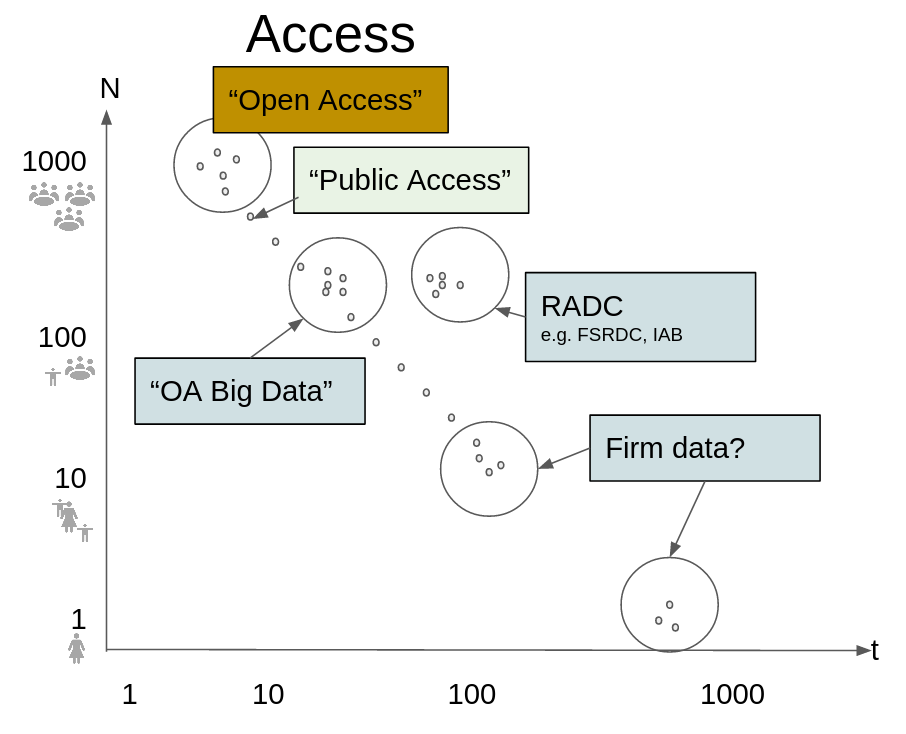
\includegraphics[width=0.8\textwidth]{figure1.png}
    \caption{Conceptual trade-off between number of individuals accessing data, and time required to do so. Figure first published in \citet{vilhuber_reproducibility_2023}.}
    \label{fig:nxt}
\end{figure}

\section{Data Access}
\label{sec:data_access}

One subcomponent of open science, and locus of much attention throughout the literature in the social sciences, are ``open data.'' This in principle easy - why should the data used in research not be open? However, the various caveats that policies and principles include are important to recognize. \parencite{open_knowledge_foundation_defining_2024} mentions ``requirements that preserve provenance and openness,'' which does not take into account privacy. \citet{unesco_understanding_2022} does note  ``human rights, security, personal privacy.'' On the other hand, even much data that is available to almost anybody on the Internet may not actually be ``open. ''  Consider the S\&P~500, viewed in newspaper and many websites \parencite[e.g.][]{sp_dow_jones_indices_llc_sp_2025}, is not ``open data'' because it does not allow for free re-use. OKF defines 
``open data'' as requiring machine readability, absence of licensing charges, and free re-use, but does not mandate availability via download on the internet, absence of all fees, nor absence of any technical measures, such as a requirement to register and agree to abide by these rules \citep{open_knowledge_foundation_defining_2024}. 

The United States government has traditionally put its data products in the public domain (i.e., without any restrictions on usage or attribution), which makes it ``open'' in the above sense. Many countries have switched their government data to default to open data \parencite{statistics_canada_statistics_2012,uk_government_open_2014}. However, many well known ``public-use'' data are not always ``open'': IPUMS has a redistribution restriction (encapsulated in ``Terms of Use'', not a license), and some geographic data by international statistical offices remain under more stringent licensing requirements in other countries (e.g., United Kingdom). 

Many well-known surveys impose redistribution and usage restrictions that are not consistent with the OKD definition. Many such redistribution restrictions apply to datasets with more detailed personal information collected through surveys, and are meant to ensure continued compliance with ethical rules of behavior, often with informed consent agreements by survey participants and local privacy laws. Notable examples include  PSID \parencite{institute_for_social_research_panel_2024}, World Value Survey \parencite{haerpfer_world_2024}, Demographic Household Surveys \parencite{dhs_program_demographic_2024}, German Socio-Economic Panel \parencite{goebel_german_2019,goebel_socio-economic_2024}, all of which have broad (cost-free) usage, conditional on registration and compliance with usage restrictions. Table~\ref{

gradations of access, ranging from "sign/click through this agreement before downloading"  to "write a paragraph about what you want to do, but don't share the data"  to "you have to put this on a secure computer and BTW obtain IRB approval for your access". In fact, authors sometimes forget to abide by these rules, and we (data editors) must sometimes remind them of it, or correct the errors after publication ("take-down requests", see <https://aeadataeditor.github.io/posts/2024-11-01-psid-requests>). In fact, I get about 12-15 take-down requests or notifications of inappropriate data publication (or use!) per year (most, luckily, affecting cases that were simply passed through prior to my tenure, but we still miss some).


The interaction between licensing, openness, and re-use has ramifications that go beyond the scope of the present article. Good guidance on licensing of scientific data by its creators can be found in \citet{stodden_enabling_2009}.


Issues:

Open Access

Restricted Access

% table of data access in AER in 2024 using internal categorization




\section{Access to Software}
\label{sec:software}

Turning to software, I will again need to define more precisely what I mean by that. I distinguish two key categories of software: \textbf{high-level interpreters} (or more rarely compilers), and \textbf{instructions}. The former will in turn comprise software used in two key but distinct features of the scientific production process: \textbf{data collection} and \textbf{analysis}. 

\textbf{High-level software} for \textbf{analysis} are the flagship software  that receive the most  focus in the social science literature. These are software products such as Stata, MATLAB, R, Julia (see Figure~\ref{fig:software}). Most of these are interpreted languages at the user level, though user-contributed packages may be compiled (R, Julia). Increasingly present is Python, which may be both compiled and interpreted; less common are purely compiled languages such as C or Fortran. We also include here dedicated \ac{GIS} software, mostly used to create maps, though some analytical tasks can also be performed. It arguably may also comprise custom plugins to other software, such as Dynare \citep{adjemian_dynare_2024,cherrier_write_2023}.


\begin{figure}
    \centering
    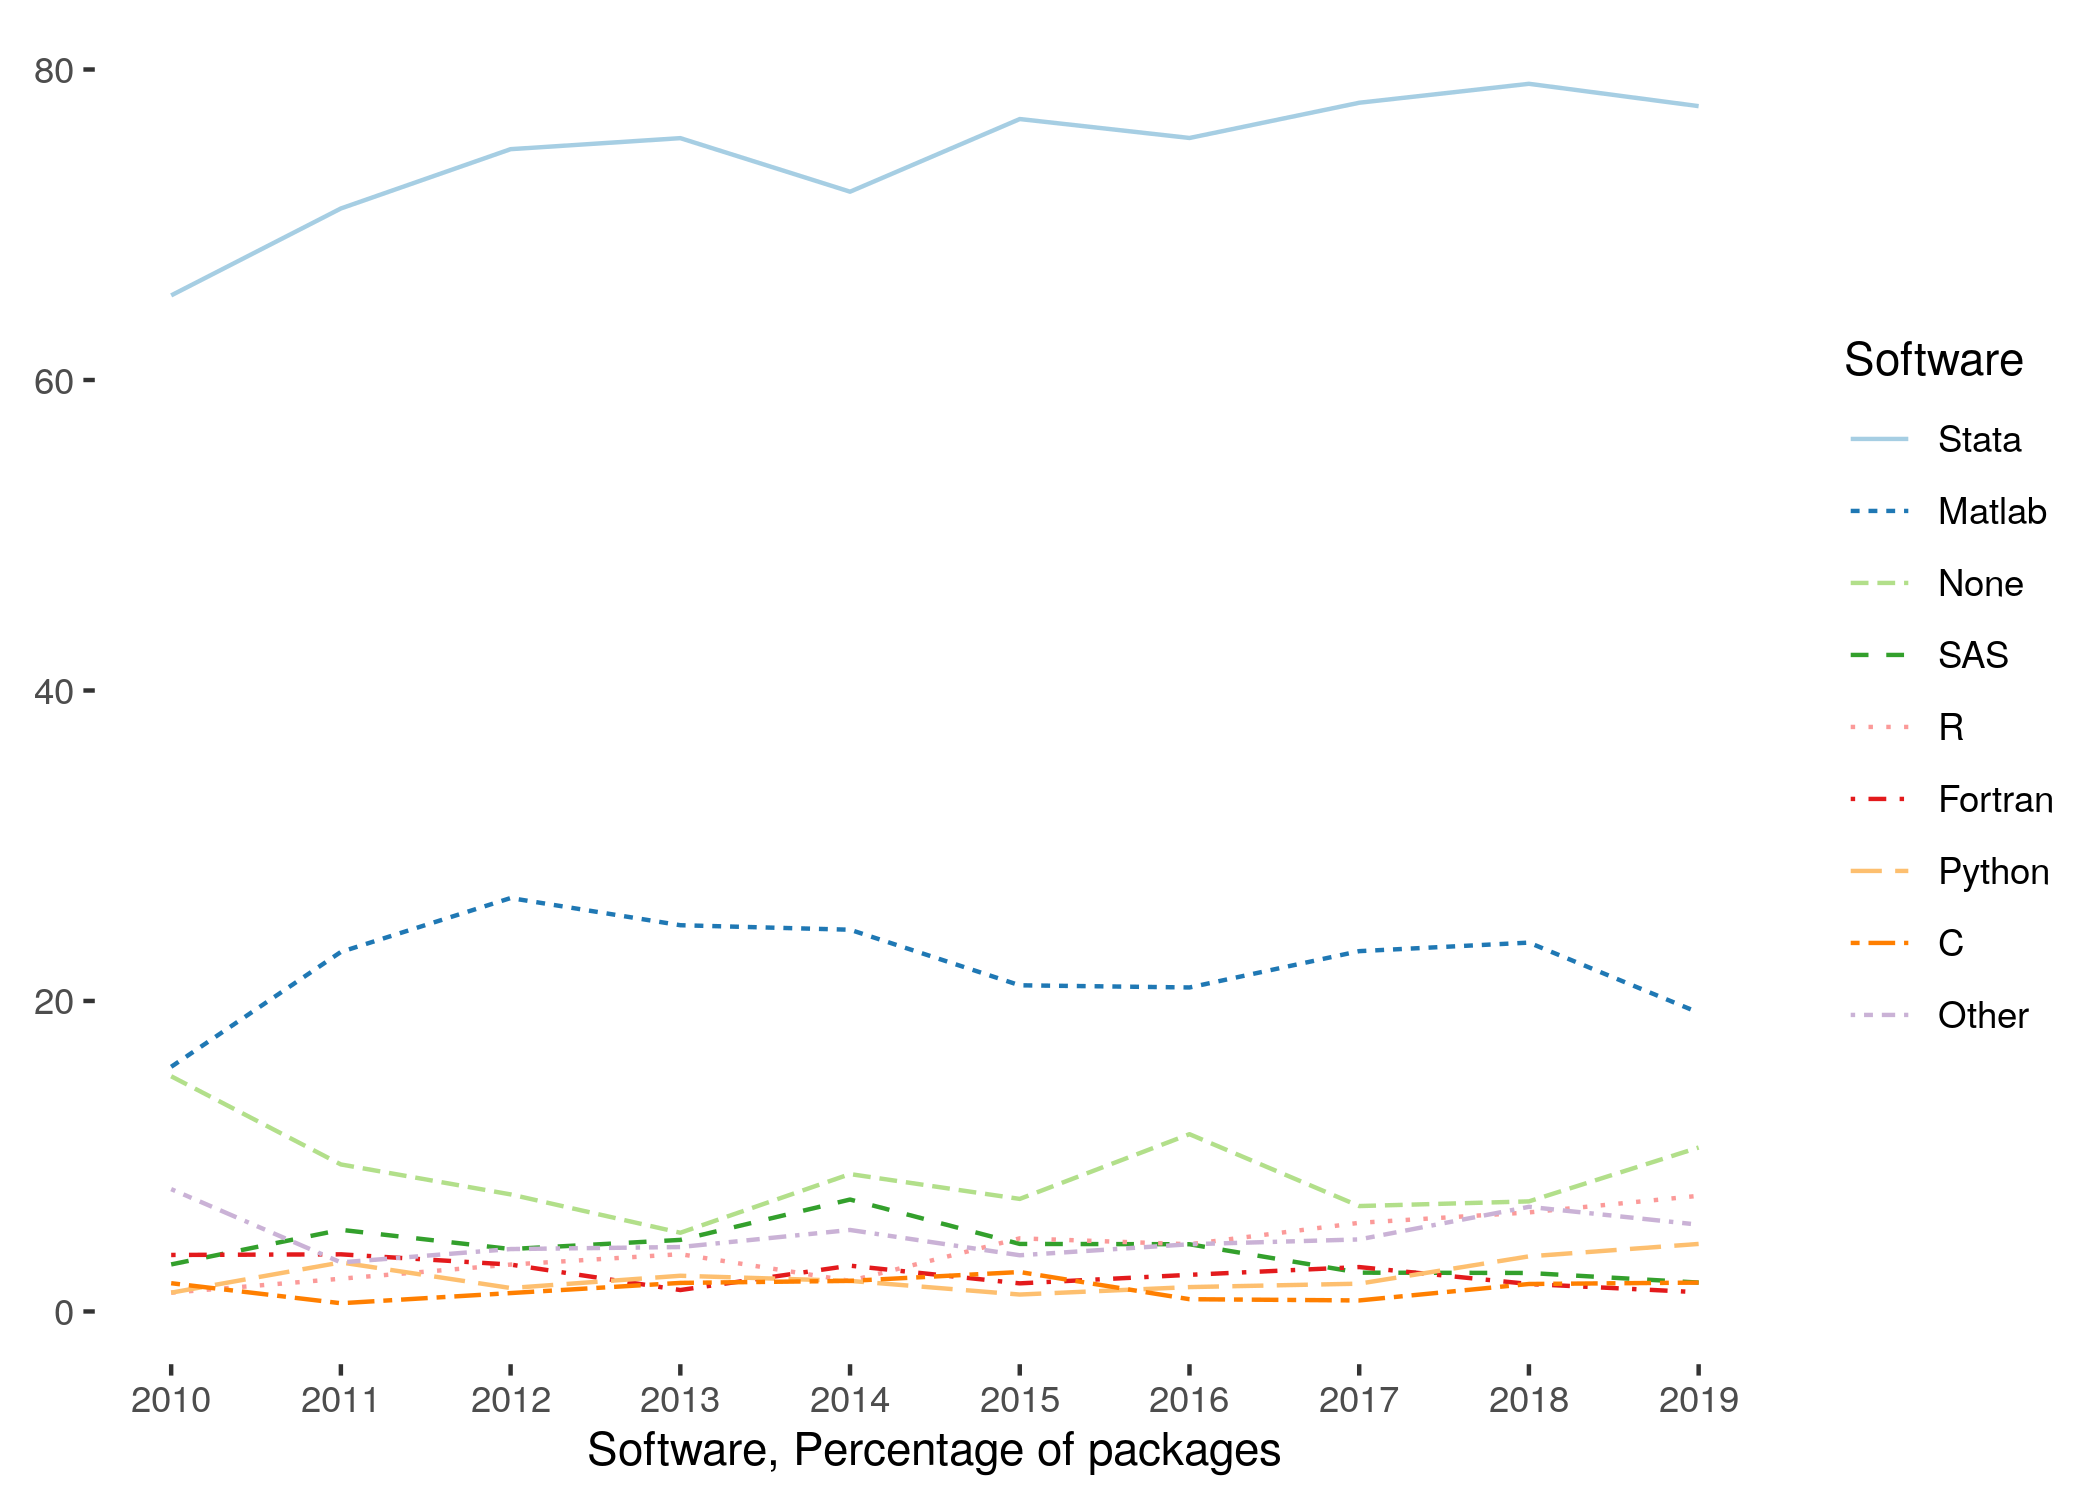
\includegraphics[width=0.8\textwidth]{pandp-2020-software-updated.png}
    \caption{Software usage in AEA journals, 2010-2019, percentage of replication packages. Data do not sum to 100\% as a replication package may use several different software. Originally published in \citet{10.1257/pandp.110.764}, corrected version see \citet{vilhuber_migrating_2020}.}
    \label{fig:software}
\end{figure}

While many economists use data collected by others, some are primary data generators or collectors, for instance through laboratory or field experiments, as well as surveys. \textbf{Data collection} software in this context are the survey software tools (Qualtrics, LimeSurvey, SurveyCTO) used to conduct surveys (including as part of lab or field experiments), as well as customized experimental software, such as oTree \citep{chen_otreeopen-source_2016} and z-tree \citep{fischbache_z-tree_2021}.

The core of a paper's analysis, however, resides in how the more general software package is manipulated, in combination with the data, via \textbf{instructions}. I do not call these `source code', as that terms tends to be used in conjunction with complex compiled software, such as those listed as \textbf{high-level software}. Rather, these instructions are mostly interpreted code, or compiled just-in-time, in the language used by the high-level software, or, as is still sometimes the case, in the form of instructions to humans on how to manipulate a non-programmed user interface for software.\footnote{In economics, this appears to occur most often for \ac{GIS} software, and sometimes for data extraction software used by data providers.}

Open access, therefore, can work through several channels. Software can have a cost. In economics, it is extremely rare to sell access to the \textbf{instructions}. However, it is quite normal for \textbf{high-level statistical software} and \textbf{data collection software} to be accessible only through purchase. As Figure~\ref{fig:software} shows, the top two statistical software products used in replication packages are commercial closed-source statistical software products: Stata and Matlab. In order to be able to re-use the instructions (code) from academic papers, a software license is required, and must be purchased. 

How much of an impediment to open access is this? Without loss of generality, to illustrate, consider Stata. An academic single-user yearly license as of January 2025 was \$690 for a US-based student. The price is the same for a student in (much poorer) Greece. For a student in Vietnam, the price drops to \$220.\footnote{See source text for data.}  To put this into perspective, the average monthly incomes in each of these countries, which students are unlikely to earn, are \$6,704, \$1,883, and \$343, respectively, and a reasonably powerful laptop a student is likely to have was around \$1,000. 


% latex table generated in R 4.3.1 by xtable 1.8-4 package
% Fri Feb  7 20:50:43 2025
\begin{table}[h]
\centering
\caption{Software licensing internationally} 
\begin{tabular}{lrrr}
  \toprule
Country & Average.monthly.income & Stata.license & Percent \\ 
  \midrule
USA & 6,704 & 690 & 10.3 \\ 
  Greece & 1,883 & 690 & 36.6 \\ 
  Vietnam & 343 & 220 & 64.1 \\ 
   \midrule \multicolumn{4}{l}{\textit{Notes:} Amounts in USD as of 2025. Source for Stata license prices: Stata website.} 
 \bottomrule
\end{tabular}
\end{table}


An informal survey of several economists working with colleagues and students in Latin America, Africa, and Asia uniformly suggested that access to commercial statistical software was often difficult for students, alleviated somewhat when students were fortunate to attend private universities. In fact, in a recent survey (CIDR), respondents were asked to name the top two factors that could support early-career African scholars’ publication success. 46\% of respondents chose 
`Providing access to datasets and data management tools' as one of the two factors. University staff and students (across multiple disciplines) were also asked which aspect they  most needed funding for, and 38\% mentioned `Data analysis software'. Within top universities, on the other hand, most researchers, including graduate students, will have access to these software products, and even many undergraduates may be able to leverage university computer labs to access these software. Outside of academia, however, it may be more constraining. Precise information is hard to come by.

The landscape is even harder to assess for \textbf{data collection software}. Open source packages otree and z-tree are often used for lab experiments. otree is cited by over by between 1,400 (OpenAlex, as of 2025-01-29) and 2,400 articles (Google Scholar, as of 2025-01-29), z-Tree is cited between 9,000 (OpenAlex) and 12,000 times (Google Scholar), but it is not clear how to benchmark that, given poor software citation practices in economics. Lab as well as field experiments will often use online survey platforms to augment experiments, or as primary data collection tool. Qualtrics, one of the big commercial platforms for surveys, is mentioned (but not cited) over 200,000 times (Google Scholar). Open source alternative LimeSurvey is mentioned about 31,000 times.

(INSERT HERE SOME INFO FROM AEA ARTICLES). 

% how to pull down the full list of Google Scholar citations, and compare to the list of top 10 journals.

The second channel is through the \textbf{instructions}. Conditional on having the right software and the appropriate resources (see next section), most economics papers have openly accessible code. The advent of data and code availability policies most certainly has helped, but also reflected attitudes already present in the researcher community.\footnote{For a review of the history of data and code availability policies in economics, see \citet{vlaeminck_dawning_2021}.} While not the first, the AEA's policy was first implemented in 2005 \citep{bernanke_editorial_2004,american_economic_association_data_2005}, but the oldest replication package curated by the AEA accompanied an 1999 article \citep{frankel_does_1999,frankel_replication_1999} preceding the policy by several years.\footnote{I believe the oldest replication package in economics may be \citet{koenker_asymptotic_1988-1}, see \url{https://aeadataeditor.github.io/posts/2023-02-02-oldest-replication-package-jae}.} While the focus of availability policies was on the data, the code often came along for the ride, albeit not always in its most complete form. The advent of newer data and code availability policies \citep[for the AEA, ][]{AEA-announcement-July-2019,AEA-announcement-July-2019}, culminating for now in multiple journals having policies compliant with \ac{DCAS} \citep{koren_data_2022}, such as the AEA \citep{american_economic_association_data_2024} and




% In line calculations
% https://www.worlddata.info/average-income.php
% US average monthly income: 6,704
% Greece: 1,883
% Vietnam:  343
%
% STata Educational single-user https://www.stata.com/order/new/edu/single-user-licenses/dl/
% Stata/MP 2-core, annual license
% US: $690
% Greece: $690
% Vietnam, Student pricing for developing economies $220


\section{Access to Other Resources}
\label{sec:other_resources}

In the template README published by myself and several other data editors in economics \parencite{templateREADMEv1.1}, we emphasize that a README should provide enough instructions for a reasonable person to re-implement the analysis described in the replication package. Here, authors need to take into account that cutting edge methods, including technology, may require more information and instruction than for standard methods. Authors likely do not need to describe how to run an analysis in Stata, given its ubiquitous use in economics, and the ease with which instructions can be found more generally, but they may need to provide detailed step-by-step information if the technology used is rare or bespoke. For instance, the emerging use of \acp{LLM} and \ac{AI} methods is far from the economic mainstream as of the writing of this article. Recent articles are still identifying ways economists scan actually use these tools, both for personal productivity \parencite{korinek_generative_2023} and as part of the technical toolkit \parencite{athey_machine_2019,dell_deep_2024}. 
%Only one of the articles submitted to any of the AEA journals in 2024 used these techniques (to be named, not yet published).

The most recent modern toolkits are not the only resource constraints that might restrict broad access. While it might be argued that the use of proprietary software is restrictive, it is one of many resource constraints that may be binding for some researchers. Researchers in lower-ranked (and lower-funded) research institutions, including in \acp{LMIC}, may well not have the funds to purchase proprietary software, but access to computers may be equally constraining. The template README requests information on the type of computer that was used by the original researcher, to provide a benchmark to future re-users. Acquiring access to sufficient memory (\ac{RAM}), storage, and use over time of those resources can be expensive, even when renting such resources in cloud environments (which very few researchers appear to be doing). Traditionally, that access may be embedded within a single purchased computer, which may have (in 2024) around 32GB of RAM, 1-2 TB of storage, and have 4-12 compute cores available exclusively to the owner. More complex analyses may require access to compute clusters (using hundreds or thousands of compute cores), very large storage arrays (measured in the two- to three-digit TB range), and may require up to 1024 GB of RAM. Cutting edge analyses may require specialized chips, such as one or more \acp{GPU}, or even a cluster of \acp{GPU}. We have observed analyses that may run data cleaning or data acquisition processes for months at a time. 

The vast majority of articles published in economics journals usually require no more computing resources than a modern laptop provides, in all the dimensions enumerated in the previous paragraph. In fact, a formal quantitative measurement of resource usage in economics articles is surprisingly hard to obtain, as most researchers are not very good at reporting the resources they have used to conduct their research. In part, this is because measuring such usage is non-trivial, but to a larger extent, I postulate that this is because most research institutions provide such resources to their researchers in a ``convenient way,'' and researchers conduct research within those constraints. More importantly, however, it suggests an important constraint on how ``open'' access can be for some if not all economics research.

Some newer research requires vastly different types of resources. Studies using raw satellite data may require more than 10TB of data storage \citep{khachiyan_using_2022,khachiyan_data_2022}, may need more than 20,000 compute hours on a cloud provider \citep{rudik_optimal_2020,rudik_data_2020}, or the use of one \citep{dell_deep_2024,dell_data_2025} or dozens \citep{khachiyan_data_2022} \acp{GPU}.\footnote{As of January 2025, the type of \ac{GPU} used by \citet{dell_data_2025}, costs between USD 4500 and USD 7700, or between 2 and 7 times as much as a standard laptop.} But  access to the code and data for these papers is open: The AEA-related replication packages for these articles are licensed under a standard \ac{CC-BY} license. Some of the data not included in the \citet{dell_data_2025} replication package is on Huggingface, also under a \ac{CC-BY} license \citep{silcock_newswire_2024}.

Are such computational constraints a problem? No consistent analysis exists that correlates resource requirements to academic outcomes such as citations, primarily because it is very hard to measure consistently the resource requirements of economic articles. The very small sample in the previous paragraph may serve to illustrate this, but without controls for scientific merit, is purely an indicator. \citet{silcock_newswire_2024} had been downloaded 98 times in December 2024, six months after the arXiv paper associated with it was published \citep{silcock_newswire_2024}. \citet{rudik_data_2020} has had  1432 views, 124 downloads for replication package, as the manuscript \citep{rudik_optimal_2020} has 15 citations. The replication package \citet{khachiyan_data_2022} has  2124 views, 175 downloads, while the manuscript \citep{khachiyan_using_2022} has 5 citations (all as of January 2025). For comparison, the average article in one of the \ac{AEA}'s journals has 908 views and 106 downloads \citep[Table 4]{vilhuber_report_2025}.

% Repository Published Downloads Views Uploads Files Size (GB)
% ICPSR 5,094 540,713 4,627,310 458 65,812 1,485.94
%
%Need: average and median number of views, downloads and citations for packages from the same year in the journals.

\section{The Benefits of Open Science in Economics}
\label{sec:benefits}

To illustrate some of the benefits of open science, I describe two recent articles in economics that leverage the availability of code and data to improve econometric methods for future researchers. The first paper relies on the empirical recomputation of prior papers to assess a theoretically ambiguous potential bias in inference. The second paper also focuses on inference, and uses actual data from previous papers to simulate the relevance of the impact. Both then provide new software (R and Stata packages), under open source licenses, to ``fix'' the problem for future studies. 

\citet{roth_pretest_2022}  uses 12 previously published papers to assess whether the usual tests for pre-existing differences in trends when using difference-in-differences methods are properly controlling for power, and the empirical impact on subsequent inference. The theoretical bias is ambiguous, so an empirical evaluation is necessary. The study both leverages the open availability of materials in economic journals, but also illustrates the limitations imposed by imperfect adherence to openness. To wit, Roth writes that he searched for 

\begin{quote}
``the phrase “event study” in papers published in the \textit{American Economic Review, American Economic Journal: Applied Economics}, and \textit{American Economic Journal: Economic Policy} between
2014 and June 2018 ... The search returned 70 total papers that include a figure that the authors describe as an event-study plot.''
\end{quote}

but continues to then be limited by lack of data in the majority of cases:

\begin{quote}
    ``I exclude 43 papers for which data to replicate the main event-study plot were unavailable. \citep[pg. 307]{roth_pretest_2022}''\footnote{He also excludes another 15 papers for reasons not related to data availability.}
\end{quote}

While it remains unclear whether the excluded papers are non-compliant with the AEA's policy at the time, or whether they have legitimate reasons not to provide the data (Roth does not provide the raw result of his search), the paper is able to make an important methodological point (723 citations as of January 2025, per Google Scholar) because it is able to fully recompute the results in previous papers, apply new tests and methodologies, and come to meaningful recommendations and tools --- Roth provides an (open source) R package to implement his methodology.

\citet{de_chaisemartin_at_2024} use open access information on RCTs (AEA registry) to find 15 RCTs of a particular type (clustered paired or small strata), of which 4 have publicly available data (and reproducible artifacts). They then provide results both on simulations using these data, and in particular, re-estimate the regressions used in those studies and apply their proposed solution, showing that the number of significant effects is reduced by one-third. In other work \citep{de_chaisemartin_two-way_2020,de_chaisemartin_difference--differences_2024}, the results from various other papers are also recomputed to empirically demonstrate the relevance of the proposed methods, and software packages \citep[e.g.][]{de_chaisemartin_chaisemartinpackagesdid_multiplegt_dyn_2025} are developed and made openly available.\footnote{Note that as of January 2025, many of the packages do not have an explicit open source license --- or any license --- applied, a common feature of economists working in the open source world. My presumption is that they simply assume that everybody knows that the code is openly available.}

In both of these examples, the ability to access prior data, code, and information is critical to improving future scientific progress, but is limited by both historical and unavoidable limitations on openness.


\section{Open Infrastructure: Publications}
\label{sec:publications}

The challenges of openly accessible written scholarship are manifold, with the current focus on ``Plan S'', master publication agreements, and in the US, similar efforts under the moniker of the ``Nelson memo'' \parencite{brainard_white_2022,brainard_us_2024}. I note that the economics profession has a very long history of making much of the written knowledge available at very low cost via working papers \parencite{vilhuber_reproducibility_2020}, with the first working papers at the reputable NBER working paper series going back to 1973 \parencite{welch_education_1973}.

At the time of this writing, I have three editorial appointments. I am the Data Editor for the journals of the \acf{AEA}, the joint executive editor for the open access and multi-disciplinary \ac{JPC}, and I am a column editor for the open access \ac{HDSR}. I will use each of these to highlight a particular pattern in broadening access to publications, without any claim to generality. 

The \ac{AEA} is a not-for-profit organization, as are many other learned societies. It self-publishes eight journals, plus the proceedings of the annual conference, without relying on a commercial publishing house. Depending on the measurement, three of these publications are in the top ten journals in economics \citep{mogstad_statistical_2022-1}. Its publication costs account for about half of its overall operating expenses, and are only partially offset by directly attributable subscription and membership fees \citep{cherry_bekaert_llp_american_2024}. In fact, 6 of the top 10 journals in economics \citep{mogstad_statistical_2022-1} are published by societies (JEL, JEP, Econometrica, AER, Restud, JOLE), some of which have as sole or primary purpose the publication of the journal.\footnote{JOLE is a bit of an outlier, in that one becomes a member of the Society of Labor Economists by subscribing to the journal, rather than the other way around.} A further three journals are primarily associated with economics departments (QJE, JPE, RESTAT), which arguably may not be driven by pure profit. The sole outlier in the top ten is the \ac{JFE}, which is owned by Elsevier, a big commercial publisher. It should be noted that the \ac{EEA} severed its relationship with Elsevier in 2003 for its official journal, creating a journal that is fully owned by the association, adding to the list of society-owned journals in economics \citep{tirole_editorial_2003}. Access to these journals is generally still on a subscription basis (JEP is the exception, being free to read), but given the primarily not-for-profit organization of its owners, personal subscriptions (often via society membership) are quite low, compared to journals in many other sciences. For instance, as of 2024, a personal subscription to the Review of Economic Studies is \$156 or €141 per annum; a yearly membership to the \ac{AEA}, providing access to the seven subscription journals and the proceedings is \$25 for students and researchers in low-income countries, and \$150 at the highest personal income tier. As outlined earlier for the AEA, these subscription fees cover only a small fraction of the production costs. Nevertheless, even these (arguably low) costs do not satisfy ``Plan S'' or ``Nelson memo'' requirements, which require no access cost to the end consumer, and in the case of ``Plan S'', also require a liberal license allowing for re-use.\footnote{``The author(s) [...] grant(s) [...] a free, irrevocable, worldwide, right of access to, and a license to copy, use, distribute, transmit and display the work publicly and to make and distribute derivative works, [...] subject to proper attribution of authorship'' \citep{max-planck-gesellschaft_berlin_2023}. }

Interestingly in the context of the previous sections, all of the society-owned journals in the previous paragraph have appointed  data (reproducibility) editors.\footnote{Two additional societies, not previously mentioned, also employ data editors: the \ac{CEA} and the \ac{WEAI}. }

Since 2018, I have been the executive editor of the \ac{JPC}, an open access multi-disciplinary journal, having taken over the journal from Stephen Fienberg \citep{vilhuber_relaunching_2018}.\footnote{Fienberg, together with Cynthia Dwork and Alan Karr, founded the journal in 2009 \citep{abowd_first_2009}. Fienberg passed away in 2016 \citep{slavkovic_remembering_2018}.  In 2023, I recruited Rachel Cummings to jointly manage the journal.} As of 2024, the journal does not charge submission fees, and is free to read (what is called ``diamond open access.'' Articles default to a Creative Commons Attribution-NonCommercial-NoDerivatives (CC-BY-NC-ND) license, though authors are allowed to choose a more liberal license, for instance to comply with ``Plan S'' (which does not allow for the ``no-derivatives'' part). As executive editor, I have been responsible for all aspects of running the journal, not just finding referees for the articles that I am responsible for. The journal is made available through open-source software called Open Journal System, hosted by its creators at \href{https://pkp.sfu.ca/hosting-services/hosting/journals/}{Simon Fraser University's Public Knowledge Project}, preserved via industry-standard mechanisms (\href{https://clockss.org/about/how-clockss-works/}{CLOCKSS}, a non-profit) in case the journal ever needs to shut down, indexed in a variety of academic indexes, including via assignment of \acs{DOI}. Copy-editing is done through a mixture of professional copy-editors and volunteer work by editors and board members. All editors, including myself, are unpaid, and referees are, like in much of the publishing industry, unpaid volunteers. Yet I do pay bills, for each of the above components of a properly managed, indexed, and preserved academic journal --- and professional copy-editors and university staff do not work for free. I am thus quite aware of the absolute minimum cost of running a (small) journal. Over the years, funding has come from a variety of chaired professorships at Carnegie Mellon (Fienberg), Cornell (Abowd), and Harvard (Dwork). In order to make such funding more robust, a non-profit society was created to better and more robustly structure the funding situation \citep{abowd_launching_2024}. Time will tell if this will stabilize the funding situation, while maintaining the foundational commitment to open access. Others, in particular \href{https://sociologicalscience.com/}{Sociological Science}, have shown that it is feasible to sustainably publish high-quality research 


\section{Conclusion}

\printbibliography[title={References}]
\end{document}


\end{document}
